\documentclass[12pt]{article}
\usepackage{tikz}
\usepackage{geometry}
\usepackage{graphicx}
\usepackage{amsmath}
 \geometry{
 a4paper,
 total={210mm,297mm},
 left=30mm,
 right=30mm,
 top=40mm,
 bottom=40mm, }
\usepackage{amssymb}
\usepackage{fancyhdr}
\pagestyle{fancy}
\lhead{USI Big Brother Team}
\rhead{Page \thepage}
\lfoot{List of Required Stuff}
\cfoot{}
\rfoot{\today}
\renewcommand{\headrulewidth}{0.4pt}
\renewcommand{\footrulewidth}{0.4pt}

\begin{document}
\title{List of Required Stuff}
\author{USI Big Brother Team}
\date{\today}
\maketitle
\section*{List}
Our intention is build a little strip board with all the sensors in as less space as possible and as much strong as possible.
\begin{itemize}
\item Sound Sensor (x3); \checkmark
\item Led Strip RGB (x2);
\item TIP 120s NPN Mosfet (x6) or something similar like (STP16NF06);
\item Photo Resistor (x10);
\item Resistor 10KOhm(x10);
\item Resistor 220Ohm(x10);
\item Jumper Red Male-Male (x5); \checkmark
\item Jumper Blue Male-Male (x5); \checkmark
\item Jumper Yellow Male-Male (x5); \checkmark
\item Jumper White Male-Male (x5); \checkmark
\item Jumper Red Male-Female (x5); \checkmark
\item Jumper Blue Male-Female (x5); \checkmark
\item Jumper Yellow Male-Female (x5); \checkmark
\item Jumper White Male-Female (x5); \checkmark
\item 2.54mm pin Male (as many as you can);
\item 2.54mm pin Female (as many as you can);
\item Strip board (x5 standard);
\item Something to cut the strip board;
\item Necessary to weld;
\item Servo (x4);
\item Big Breadboard (x1); \checkmark
\item Standard Arduino 5v Button (x5);
\item Temperature Sensor lm35 (x5);
\item Peer Motion Sensor (x2); \checkmark
\item Raspberry pi; \checkmark
\item Wifi connector for Arduino; \checkmark

\end{itemize}
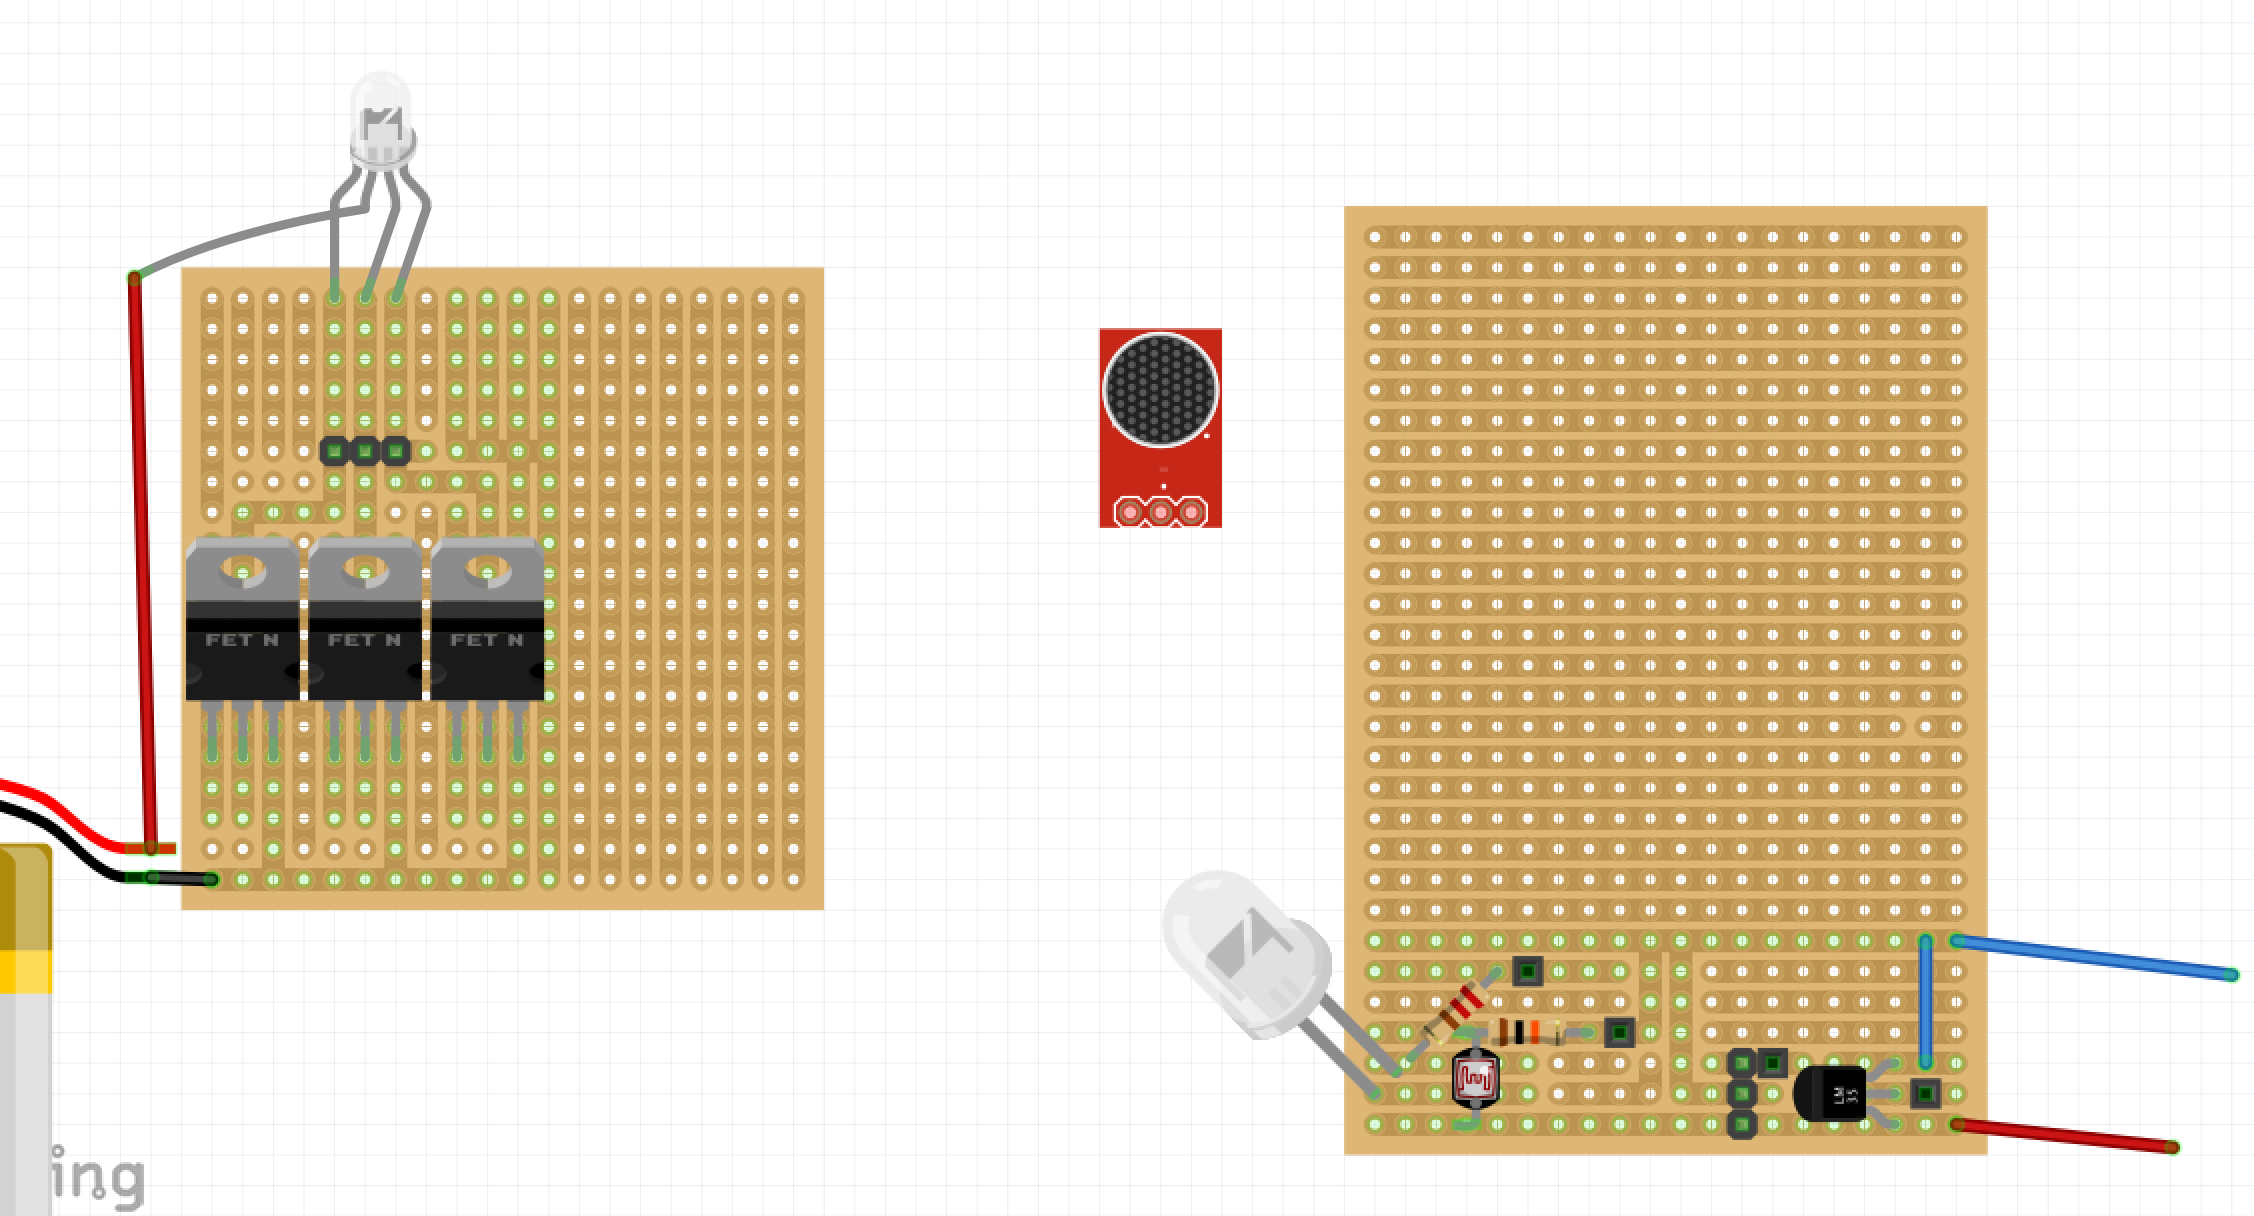
\includegraphics[scale=0.5]{stripBoard}
\end{document}